\section{}
A gas is contained in a vertical, frictionless piston-cylinder device. The piston has a mass 
of 5 kg and a cross-sectional area of 35 cm$^2$. A compressed spring above the piston exerts a 
force of 75 N on the piston. If the atmospheric pressure is 95 kPa, determine the pressure inside 
the cylinder.

\begin{figure}[h]
    \centering
    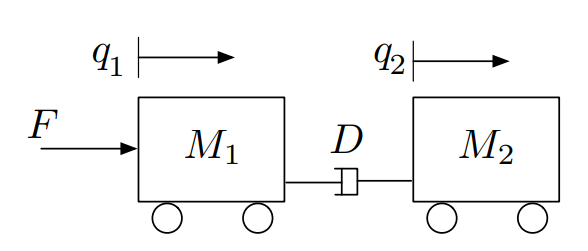
\includegraphics[width=0.3\textwidth]{Questions/Figures/Q2ProblemDiagram.png}
    \caption{Piston-cylinder device}
    \label{fig:Q2ProblemDiagram}
\end{figure}

The freebody diagram is:
\begin{figure}[h]
    \centering
    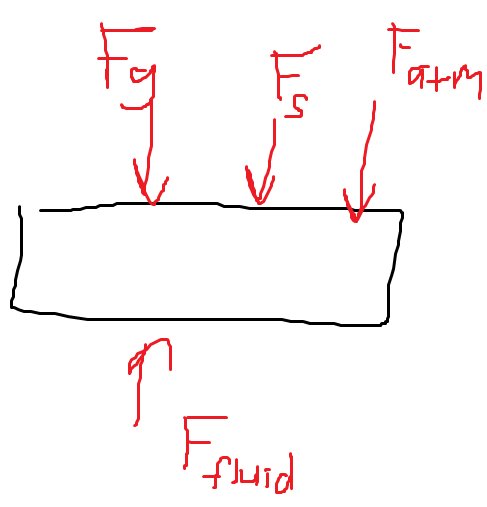
\includegraphics[width=0.25\textwidth]{Questions/Figures/Q2FBD.png}
    \caption{Freebody diagram of the piston}
    \label{fig:Q2FreeBodyDiagram}
\end{figure}

The force balance is:
\begin{align}
    F_{fluid} &= F_{s} + F_{atm} + F_{g}\\
    P_{fluid}A_{p} &= F_{s} + P_{atm}A_{p} + mg\\
    P_{fluid} &= \frac{F_{s}}{A_{p}} + P_{atm} + \frac{mg}{A_{p}}\\
\end{align}

Substituting values:
\begin{align}
    P_{fluid} &= \frac{75}{0.0035} + 95000 + \frac{5\times9.81}{0.0035}\\
            &= \qty{130442.857143}{\pascal} \\
            &= \boxed{\qty{130.4}{\kilo\pascal}}
\end{align}